\section{introduction}
Sudoku is a logic-based, combinatorial number-placement puzzle.
In classic sudoku, the objective is to fill a $9*9$ grid 
with digits so that each column, each row, and each of 
the nine $3*3$ subgrids that compose the grid contain all 
of the digits from 1 to 9. 
The puzzle setter provides a partially completed grid, which for a well-posed puzzle has a single solution.

Completed games are always an example of a Latin 
square, including an additional constraint on the 
contents of individual regions. For example, the 
same single integer may not appear twice in the 
same row, column, or any of the nine $3*3$ subregions 
of the $9*9$ playing board.
\begin{figure}[H]
    \centering
    \begin{tabular}{p{0.5\textwidth}p{0.5\textwidth}}
    \subfloat[example of a sudoko puzzle]{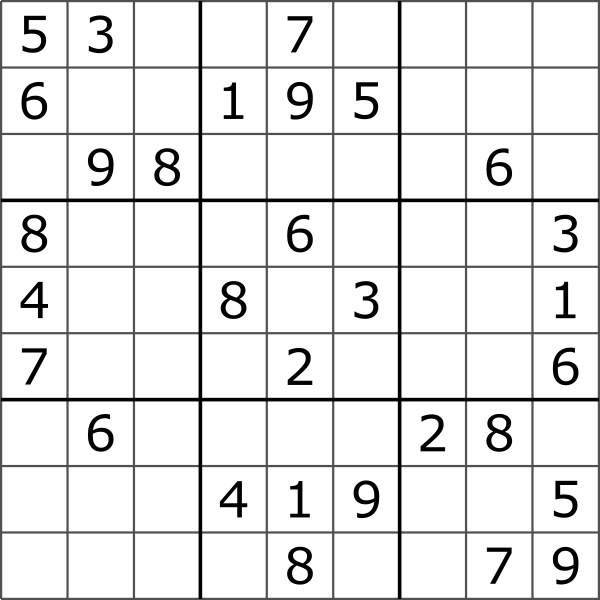
\includegraphics[width=0.5\textwidth]{images/sudoku.png}} &
    \subfloat[corrosponding solution of the puzzle of (a)]{ 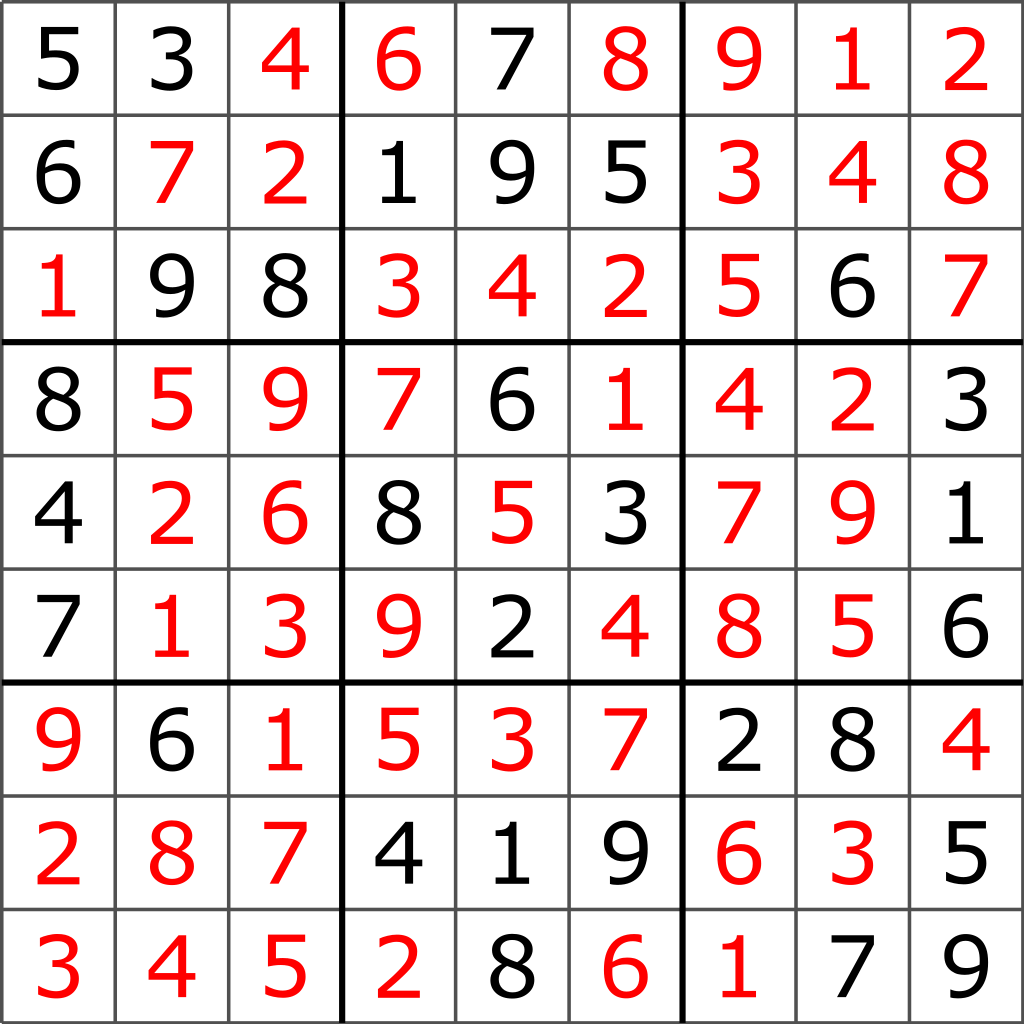
\includegraphics[width= 0.5\textwidth]{images/sudoku2.png}}
    \end{tabular}
\end{figure}